\documentclass[12pt]{beamer}
\usepackage{amsmath,amssymb,caption,float,hyperref,tabularx}
\usepackage{minted}  % Use minted instead of listings
\usepackage[ruled,vlined]{algorithm2e}
\usepackage[utf8]{inputenc}
\usepackage[english]{babel}
\usepackage{biblatex,csquotes}
\addbibresource{p3pre.bib}
\captionsetup[figure]{labelsep=period}
% \captionsetup[table]{labelsep=period}
\definecolor{bg}{rgb}{0.95,0.95,0.95}
\hypersetup{
    colorlinks=true,
    linkcolor=blue,
    filecolor=blue,      
    urlcolor=blue,
    citecolor=cyan,
}
\usemintedstyle{emacs}
\usetheme{Madrid}
\setbeamercolor{normal text}{bg=black!10}

\SetKwInOut{Input}{Input}
\SetKwInOut{Output}{Output}
\SetKwProg{Fn}{Function}{\string:}{end}
\SetKwFunction{parse}{parse}

\begin{document}
\title{Minix 3.2.1 User Space \& Kernel Space}
\subtitle{VE482 Project3 Presentation}
\author[Group 2]{Group 2\\Haoran Jin, Yihua Liu, Yu Xiao, Yuxiang Zhou}
\institute{UM-SJTU Joint Institute}
\date{\today}
\begin{frame}
    \titlepage
\end{frame}
\section{Overview}
\begin{frame}{Overview}
\begin{itemize}
    \item Kernel Space
    \item User Space
    \begin{itemize}
        \item Drivers
        \item Servers
        \item User-land libs and exes
    \end{itemize}
\end{itemize}
\begin{figure}[H]
    \centering
    \includegraphics[width=0.4\linewidth]{overview.png}
    \caption{Overall architecture \cite{pessolani2011minix}.}
    \label{fig:overview}
\end{figure}
\end{frame}
\section{Kernel Space}
\begin{frame}{Micro-Kernel}
Minix 3 is a POSIX-compatible operating system.
\begin{itemize}
    \item a micro-kernel running a collection of multiple user-mode server processes.
    \item achieve high reliability
    \item observing the principle of least authority by limiting what each process has access to and what they can do
\end{itemize}
\end{frame}
\begin{frame}{Kernel Space}
    Low-level functionality
    \begin{itemize}
        \item interrupt
        \item scheduling
        \item a primitive form of process
        \item inter-process communication
        \begin{itemize}
            \item message passing
            \item memory grants
        \end{itemize}
    \end{itemize}
\end{frame}

\begin{frame}{Kernel System Call}
\begin{itemize}

    \item Provided by micro-kernel and specific to Minix
    \item allow the rest system to access message passing, message grants and the hardware
    \item not POSIX system call(They are implemented at a higher abstraction level)
         
\end{itemize}
\end{frame}
\begin{frame}[fragile]{The Code for Kernel Space}

\begin{itemize}
    \item Kernel source files: \texttt{/usr/src/kernel}

    \item Kernel API: \texttt{/usr/src/lib/syslib}
    
\end{itemize}
        \begin{figure}[!htb]
	\centering
	\includegraphics[scale=0.12]{kernel.png}
	\caption{Minix kernel files.}
	\label{fig:png_a}
\end{figure}
\end{frame}

\section{User Space}
\begin{frame}{Drivers}
    Drivers are software components used to manage hardware peripherals\cite{minixdriver}.
    \begin{itemize}
        \item Each driver runs as a separate user-land process and has the controls of some I/O devices.
        \item Drivers can be categorized into two types:
        \begin{itemize}
            \item Block Device Drivers
            \item Character Device Drivers
        \end{itemize}
        \item Minix drivers are processes that have permission to access their I/O ports through micro-kernel (kernel calls).
        \item Minix drivers protocol:
        \begin{itemize}
            \item The Block Device Protocol
            \item The Data Link (inet-ethernet) Protocol
            \item The I2C Device Protocol
            \item The RTC Protocol
        \end{itemize}
    \end{itemize}
\end{frame}

\begin{frame}{Source Code of Drivers}
    The source code of drivers: \texttt{/usr/src/drivers}
    \begin{figure}[H]
        \centering
        \includegraphics[width=0.9\linewidth]{drivers.png}
        \caption{drivers files}
        \label{fig:drivers_png}
    \end{figure}
\end{frame}

\begin{frame}{Servers}
The servers processes servers the other part of the operating system. Different from drivers, servers cannot directly access to hardware resources. Minix servers include the virtual memory, virtual file system, actual file systems, network stack, and data store servers \cite{minixarch}. We will mainly introduce two components: VM (Virtual Memory Manager) and VFS (Virtual File System). The source code of servers are under \texttt{/usr/src/servers}.
\begin{figure}[H]
    \centering
    \includegraphics[width=0.9\linewidth]{servers.png}
    \caption{servers files}
    \label{fig:servers_png}
\end{figure}
\end{frame}

\subsection{Virtual Memory Manager}
\begin{frame}{Servers}{Virtual Memory Manager}
    Virtual Memory Manager (VM) manages the usage of the memory in the operating system. There are important data structures in VM describing the memory a process is using in detail\cite{minixVM}:
    \begin{itemize}
        \item Regions: a contiguous range of virtual address space that has a particular type and some parameters described by \texttt{struct vir\_region} or \texttt{region\_t}
        \item Physical regions: a structure exist to reference physical blocks described by \texttt{struct phys\_region}
        \item Physical blocks: a single page of physical memory described by \texttt{struct phys\_block}
        \item Memory type: abstraction of different behaviour of different memory types described by \texttt{struct mem\_type}
    \end{itemize}
\end{frame}
\subsection{Virtual File System}
\begin{frame}{Servers}{Virtual File System}
    Virtual File System is an abstract layer on top of actual file systems, allowing client applications to access different types of file systems. It provides an interface between the kernel and the file systems, \cite{vfswikipedia}. It can handle most POSIX system calls including:\\    \texttt{access, chdir, chmod, chown, chroot, close, creat, fchdir, fcntl, fstat, fstatfs, fstatvfs, fsync, ftruncate, getdents, ioctl, link, llseek, lseek, lstat, mkdir, mknod, mount, open, pipe, read, readlink, rename, rmdir, select, stat, statvfs, symlink, sync, truncate, umask, umount, unlink, utime, write.}\\
    It also maintains process states shared with PM and VM and keeps track of endpoints that are supposed to be special files of character devices or block devices \cite{vfsinternal}.
\end{frame}
\begin{frame}{Servers}{Virtual File System}
\begin{figure}[H]
    \centering
    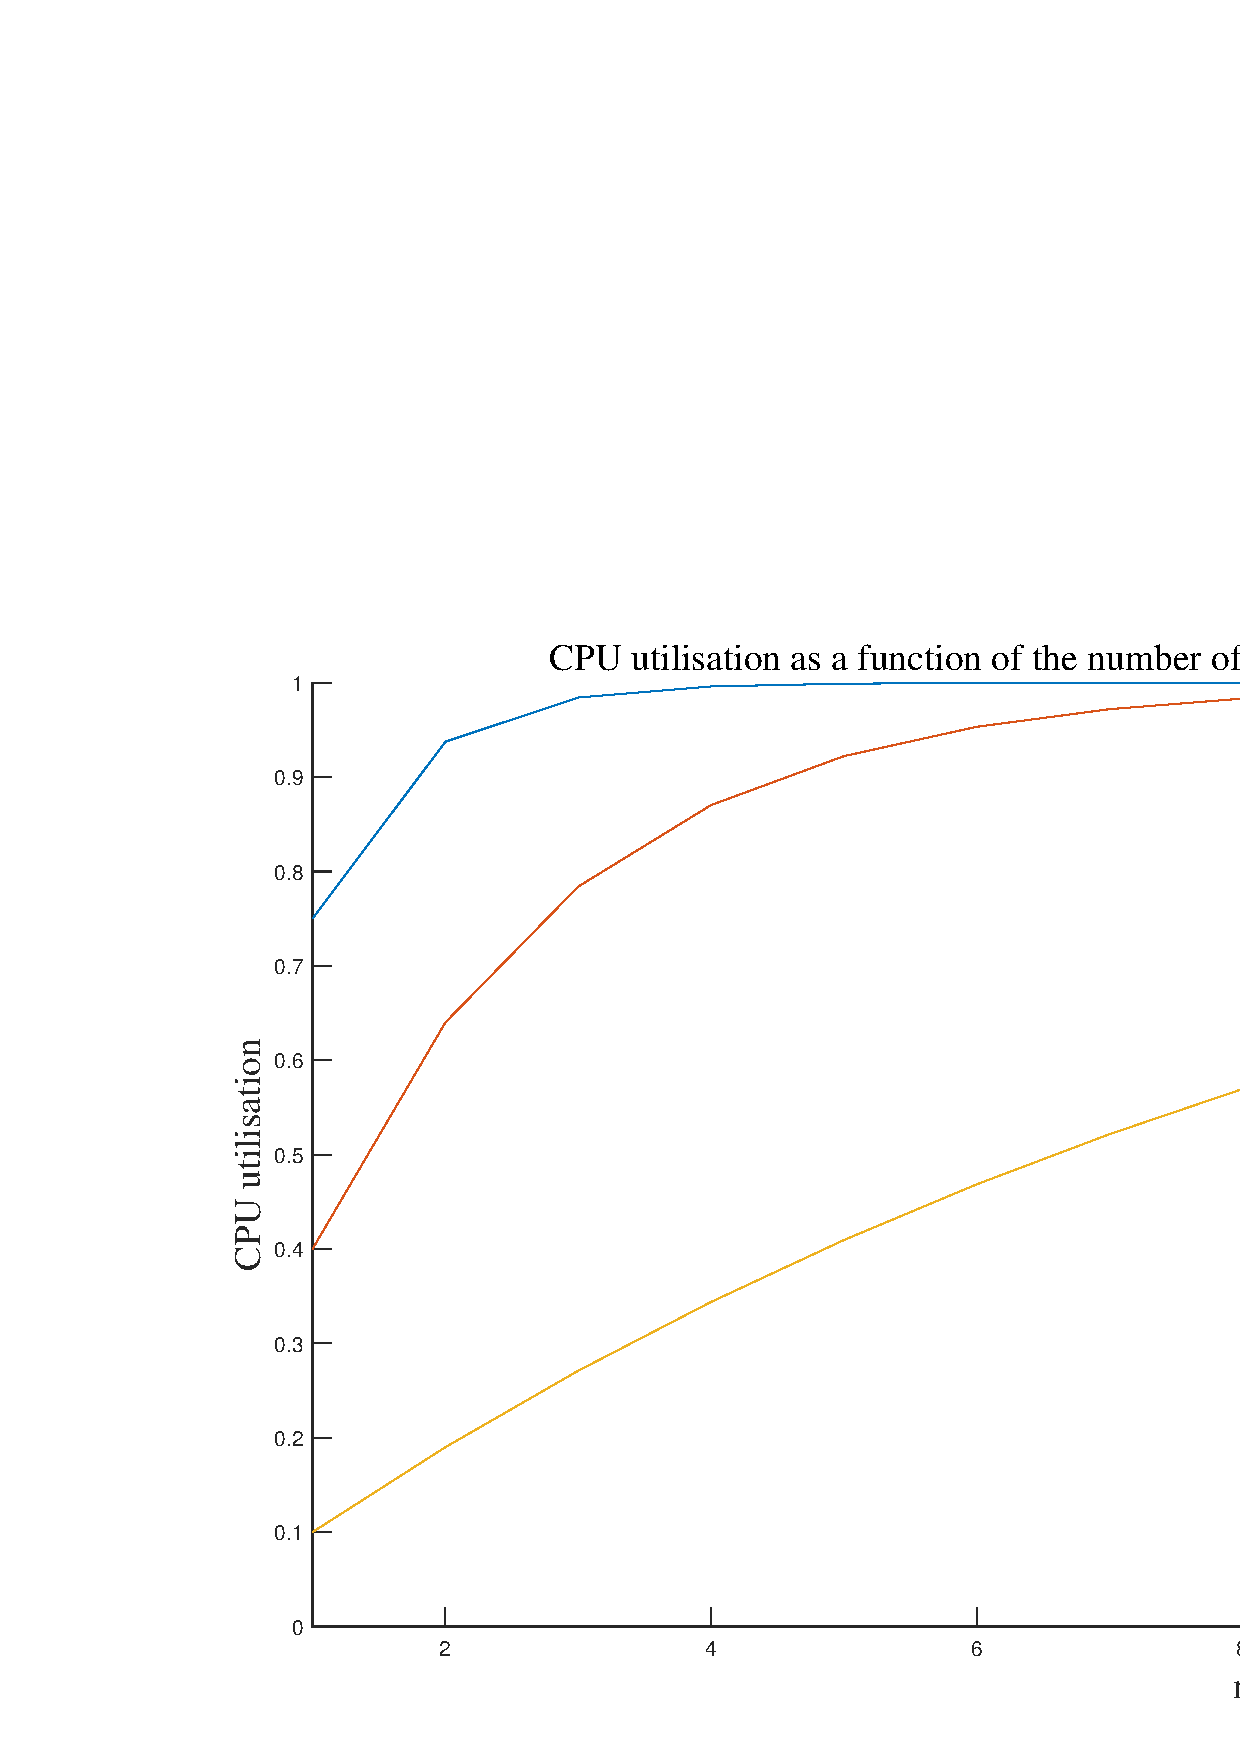
\includegraphics[width=0.8\textwidth]{1.pdf}
    \caption{Handling of \texttt{read(2)} system call.}
\end{figure}
\end{frame}

\subsection{Other Types of Servers}
\begin{frame}{Servers}{Other File System Servers}
\begin{itemize}
   \item \texttt{pfs}: Pipe File System server. Starting from Minix 3.1.6, pipe handling is removed from file-system drivers to PipeFS.
    \item \texttt{mfs}: Minix File System server. It consists of boot block, superblock, inode bitmap, zone bitmap, inodes area, and data area. It enlightened Linux Torvalds' Extended File System (\texttt{ext}).
    \item \texttt{procfs}: Process File System server (starting from Minix 3.2.0). It presents information about processes and other system information as a hierarchical file-like structure widely adopted by Linux, OpenBSD, Solaris, etc \cite{procfswikipedia}. In Minix 3, its internal is a \texttt{VTreeFS}, which organization index nodes as a tree by \texttt{struct fs\_hooks} and \texttt{struct inode\_stat}. However, security-sensitive information is not dealt with because malicious program may obtain secure values that they should not have permission to \cite{procfsnotes}.
\end{itemize}
\end{frame}
\begin{frame}{Servers}{Other File System Servers}
\begin{itemize}
    \item \texttt{ext2}: second extended file system. Support added since version 3.1.8.
    \item \texttt{hgfs} file system. Support added since version 3.1.6. \texttt{hgfs} is supported for mounting VMware shared folders as file system.
    \item \texttt{vbfs} file system. Support added since version 3.2.1. \texttt{vbfs} is supported for mounting VirtualBox shared folders as file system.
    \item \texttt{iso9660fs}: ISO 9660 file system. It is used to manage optical disc media.
\end{itemize}
\end{frame}
\begin{frame}{Servers}{Other Types of Servers}
There are also other types of servers, such as \cite{srvdrvoverview}
\begin{itemize}
    \item \texttt{rs}: Reincarnation Server. Reincarnation server is a special feature of Minix 3. \footnote{Minix 3 is now dedicated to become a very reliable and safe operating system. Prof. Tennabaum believes that his work is only completed when any users will not get themselves into trouble of system crash \cite{mos4chn}.} It is used to monitor and periodically pings all the drivers and restart them automatically if they crash. It can also kill and restart the looping drivers (making a fresh copy) if they got into an infinite loop and is not responding to status requests \cite{minix3wikipedia}. Both problems cannot be solved in monolithic designs.
    % https://tex.stackexchange.com/questions/99452/biblatex-origlanguage-field-and-output-customization
    % 4.9.2.18 Language Names of biblatex documentation, Chinese is not supported as 'langchinese', so use literal 'Chinese' instead
    \item \texttt{ds}: Data Store Server. It is used to store states and retrieved later. For example, \texttt{rs} can make use of it after a crash and subsequent restart \cite{ds}.
\end{itemize}
\end{frame}
\begin{frame}{Servers}{Other Types of Servers}
\begin{itemize}
    \item \texttt{pm}: Process manager.
    \item \texttt{sched}: Scheduler server.
    \item \texttt{is}: Information server. It is used to debug dumps.
    \item \texttt{ipc}: System V IPC server. It works parallel to native minix IPC in kernel.
    \item \texttt{inet} and \texttt{lwip}: TCP/IP protocol stack server.
    \item \texttt{init}: Parent of all user processes.
    \item \texttt{devman}: Device manager for hot-plugging of hardware (with \texttt{devmand} daemon).
\end{itemize}
\end{frame}

\section{User-land libs and exes}
\begin{frame}{User-land libs and exes}
    The userland is the collection of libraries and executables that can be used by the users of the operating system, ranging from basic system utilities to desktop environments, web browsers and video games\cite{minixuserland}. 
    \begin{itemize}
        \item Since Minix 3.2.0, Minix has imported huge amounts of userland from the NetBSD project, including bootloader, libc, various utilities and other libraries\cite{minix3wikipedia}.
        \item Basically, all the directories in \texttt{/usr/src} except for \texttt{/usr/src/kernel}, \texttt{/usr/src/drivers}, and \texttt{/usr/src/servers} belongs to the userland.
    \end{itemize}
\end{frame}

\begin{frame}{User-land libs and exes}
    You may find system utility \texttt{gcc} in \texttt{/usr/src/tools}, system utility \texttt{cd} in \texttt{/usr/src/commands}, and system utility \texttt{ls} in \texttt{/usr/src/bin}.
    \begin{figure}[H]
        \centering
        \includegraphics[width=0.9\linewidth]{userland.png}
        \caption{directory of userland}
        \label{fig:userland_png}
    \end{figure}
\end{frame}
\section{Reference}
\begin{frame}[allowframebreaks]{Reference}
    \printbibliography
\end{frame}
\section{Thanks}
\begin{frame}
\begin{center}
    \Huge Thanks!
\end{center}
\end{frame}
\end{document}
